\section*{2 \"Ubung (Abgabe: 22.04.2010, 8.30 Uhr, schriftlich)}

\subsection*{1. Gegeben sei eine periodische Funktion \"uber die Zeit, wie lauten die Fourierkoeffizienten?}
a) $f(t) = \sin(t)~\text{f\"ur}~t \in (-\pi, \pi)$\\
$a_0 = 0; ~ a_k = 0; ~ b_k = 1; ~ k = 1$\\\\
b) $f(t) = \cos(t)~\text{f\"ur}~t \in (-\pi, \pi)$\\
$a_0 = 0; ~ a_k = 1; ~ b_k = 0; ~ k = 1$\\\\
c) $f(t) = \cos(2t)~\text{f\"ur}~t \in (-\pi, \pi)$\\
$a_0 = 0; ~ a_k = 1; ~ b_k = 0; ~ k = 2$\\\\
d) $f(t) = 1~\text{f\"ur}~t \in (-\pi, \pi)$\\
$a_0 = 2; ~ a_k = 0; ~ b_k = 0; ~ k = 1,2,3...$

\subsection*{2. Gegeben seien die Fourierkoeffizienten einer Funktion \"uber die Zeit. Wie lautet die Funktion?}
Siehe Abbildungen \ref{fig:2.2.a},  \ref{fig:2.2.b} und \ref{fig:2.2.c}.
\begin{figure}[p] %  figure placement: here, top, bottom, or page
   \centering
   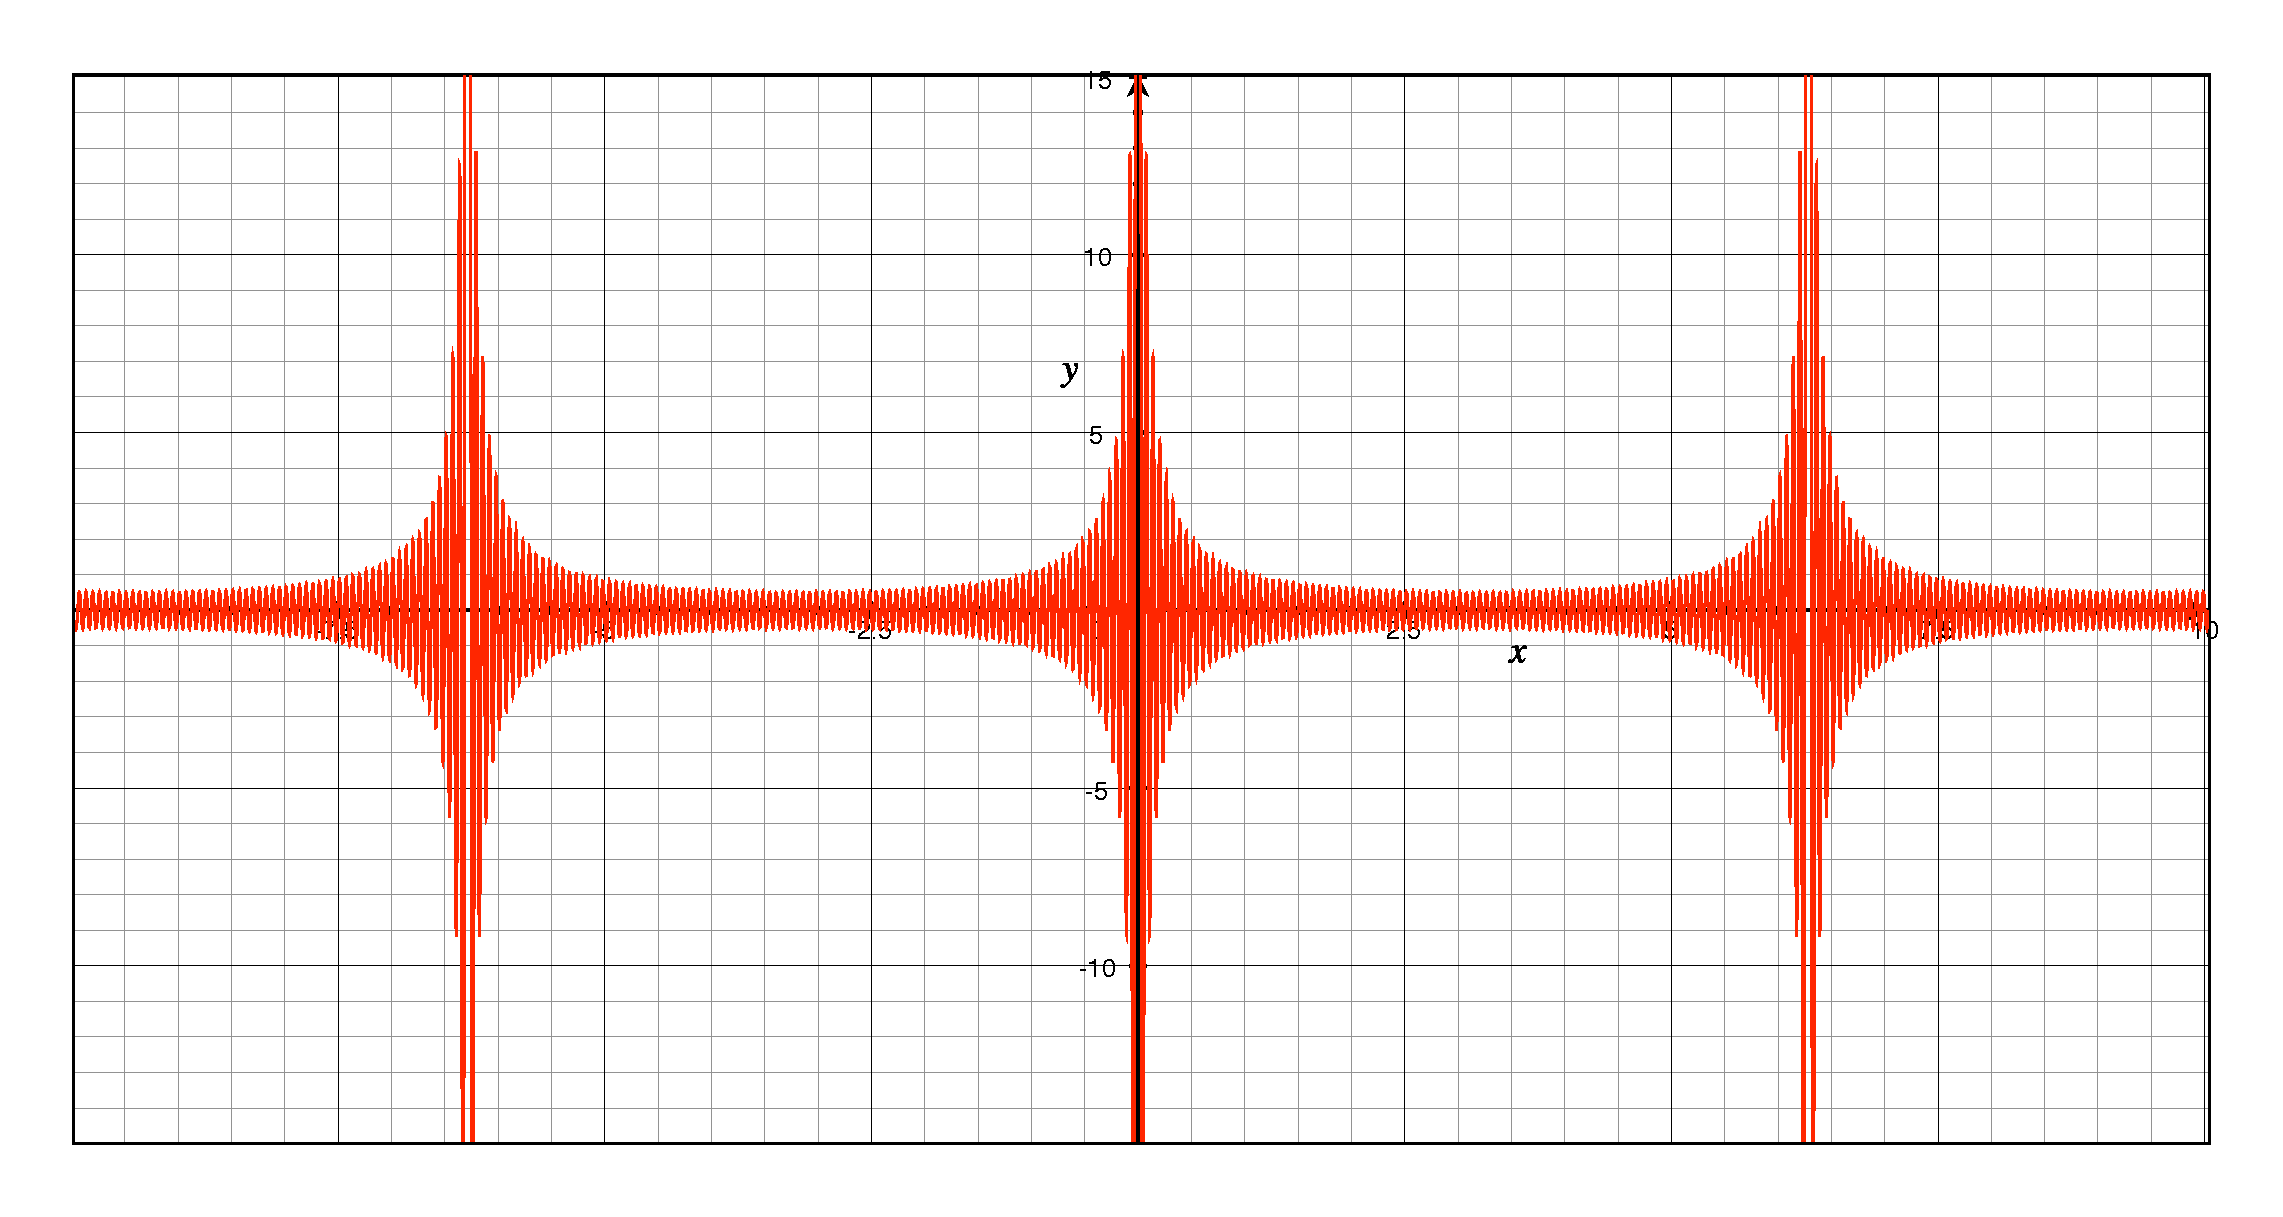
\includegraphics[width=0.4\textheight]{Uebung2/Aufgabe_2_2_a.pdf} 
   \caption{$f(x)=\frac{1}{2}+\sum_{k=1}^n cos(kx), n=100$}
   \label{fig:2.2.a}
\end{figure}
\begin{figure}[p] %  figure placement: here, top, bottom, or page
   \centering
   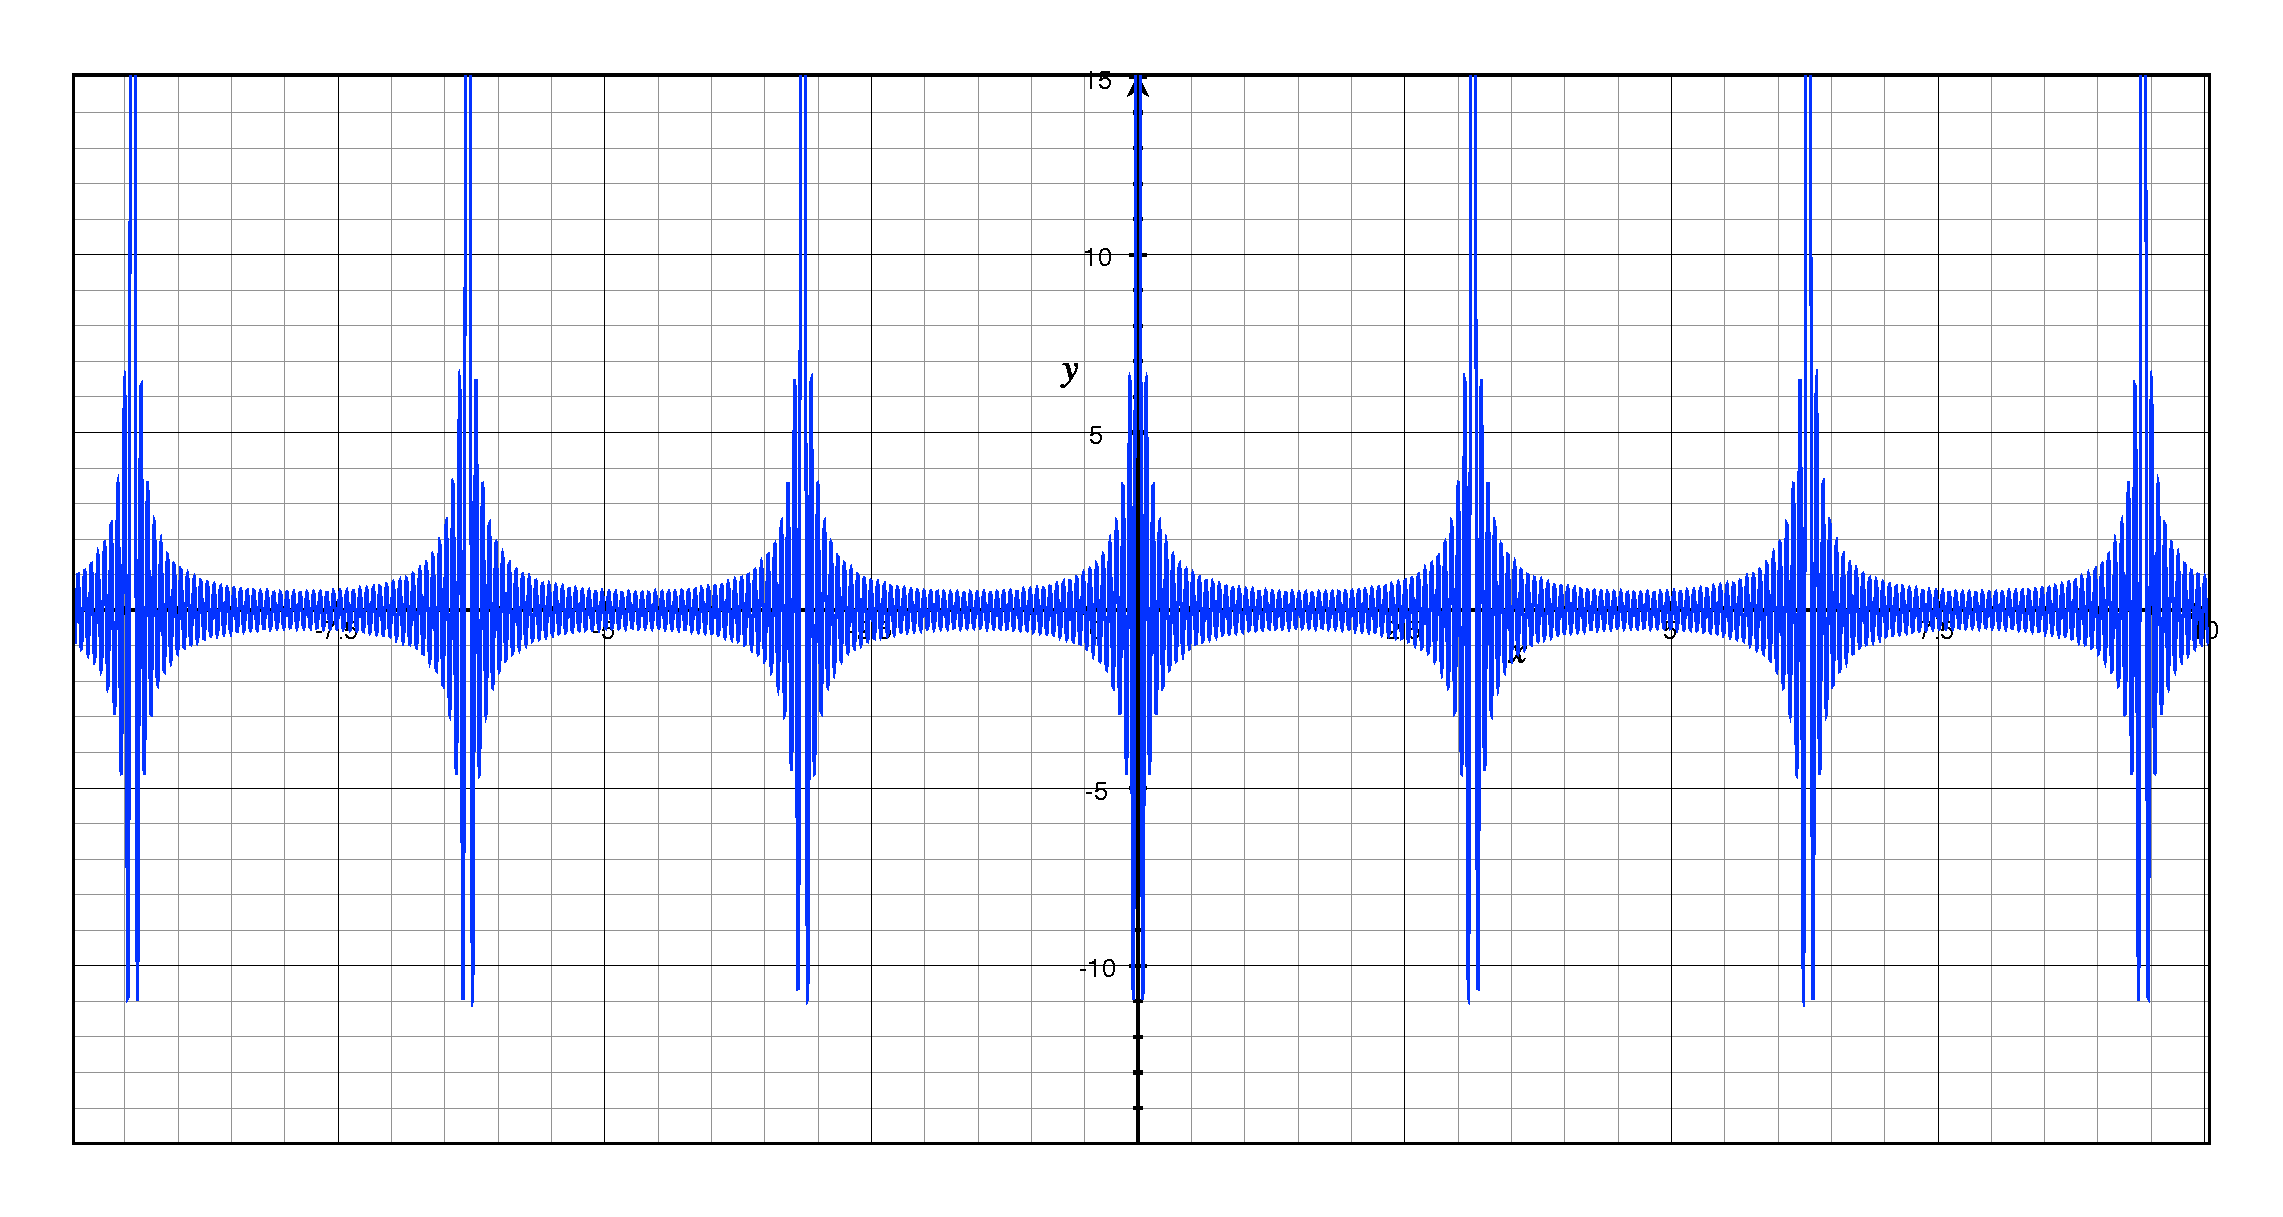
\includegraphics[width=0.4\textheight]{Uebung2/Aufgabe_2_2_b.pdf} 
   \caption{$f(x)=\frac{1}{2}+\sum_{k=2i}^n cos(kx), n=100, i=1,2,3...$}
   \label{fig:2.2.b}
\end{figure}
\begin{figure}[p] %  figure placement: here, top, bottom, or page
   \centering
   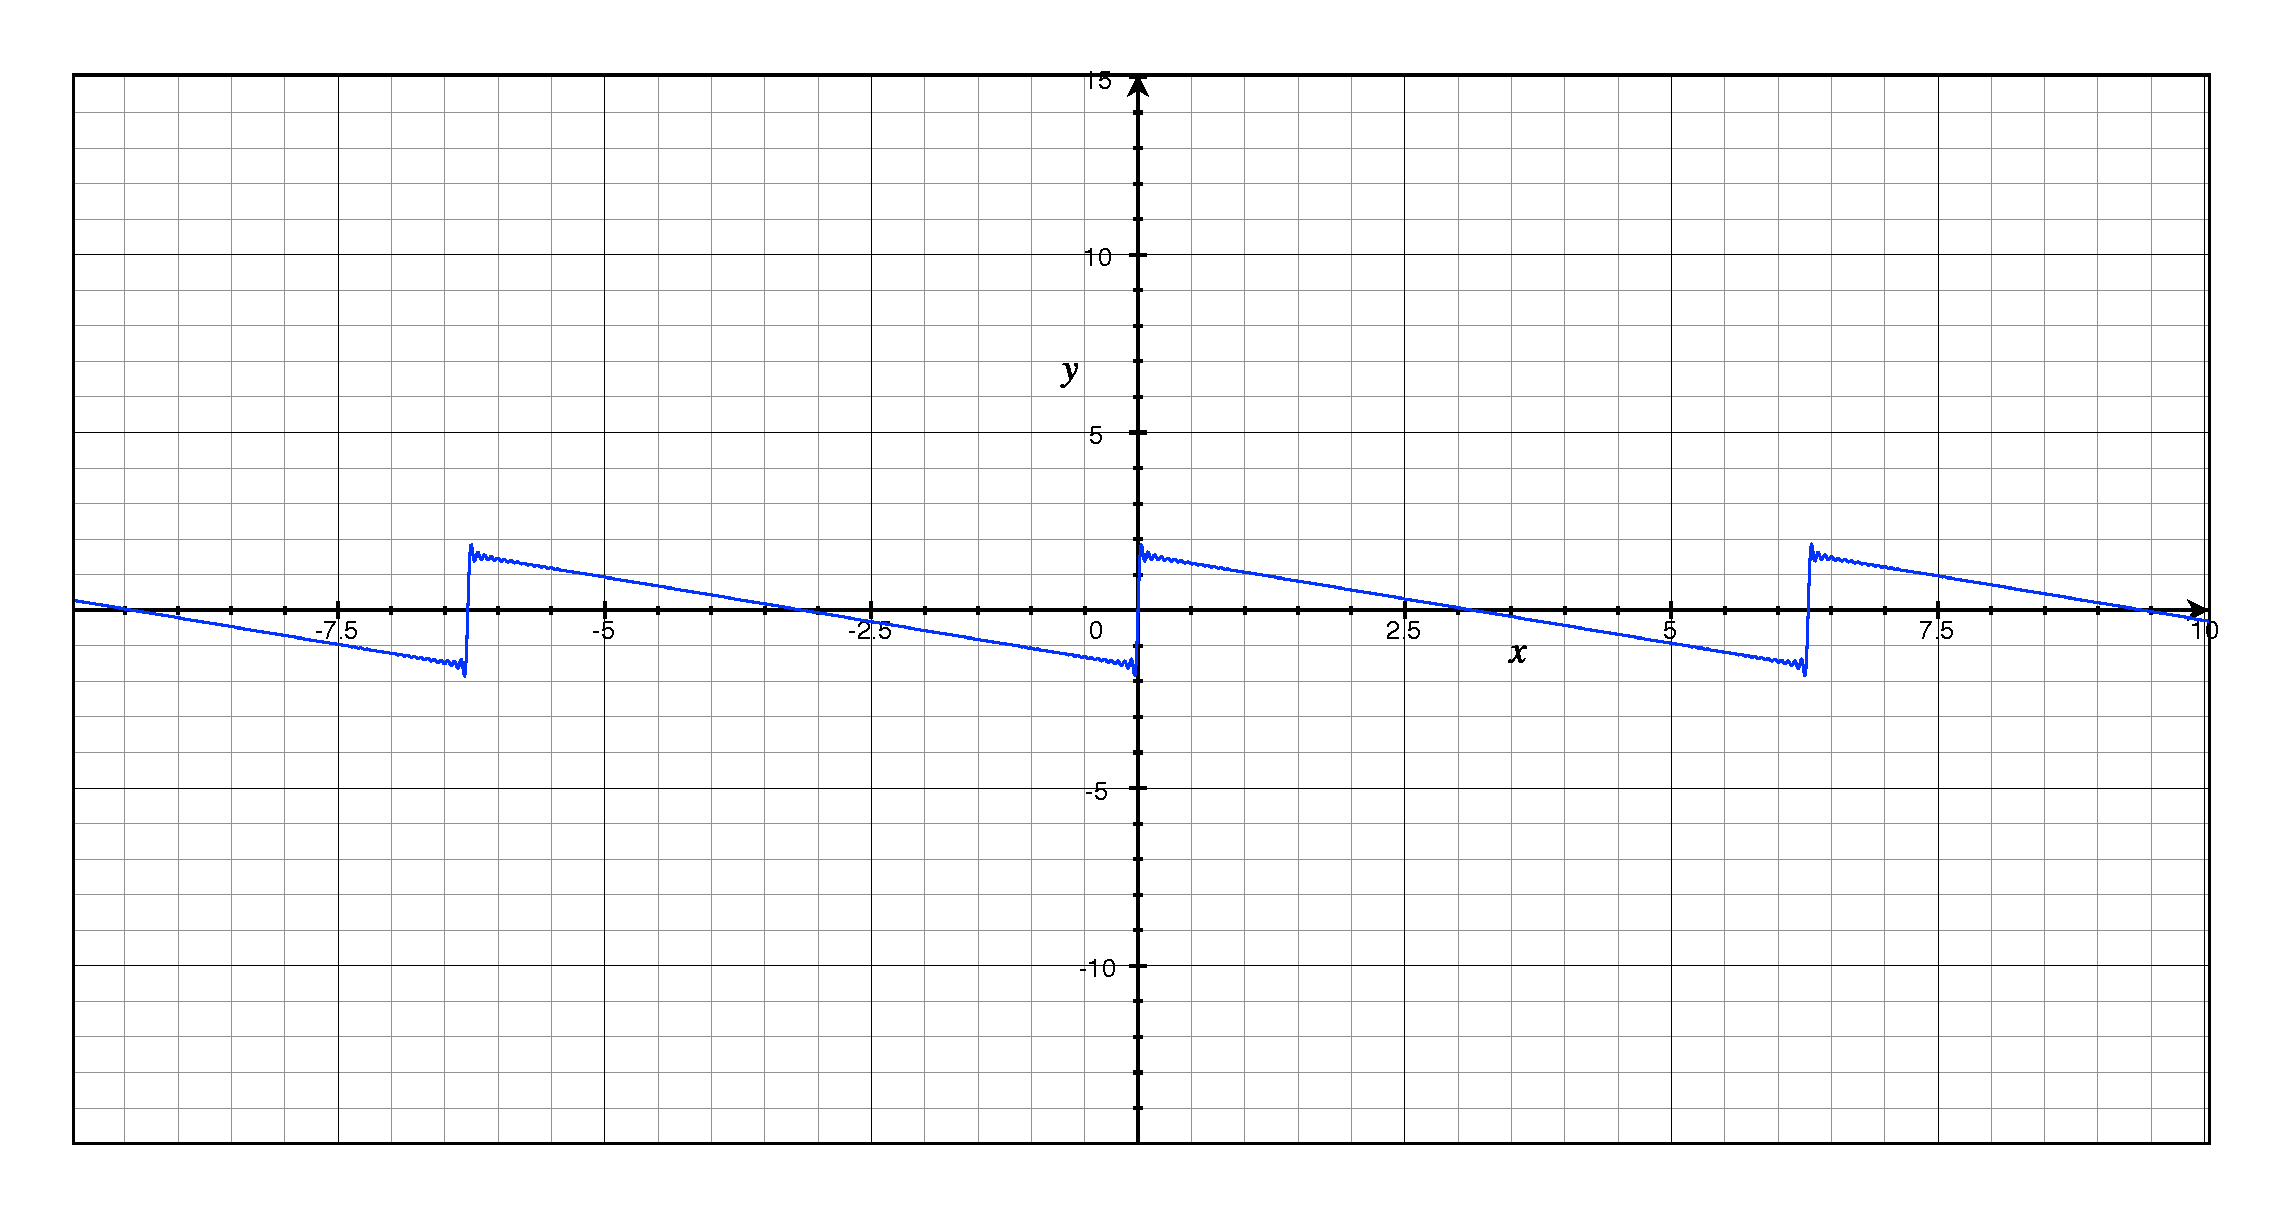
\includegraphics[width=0.4\textheight]{Uebung2/Aufgabe_2_2_c.pdf} 
   \caption{$f(x)=\sum_{k=1}^n \frac{1}{k}sin(kx), n=100$}
   \label{fig:2.2.c}
\end{figure}

\subsection*{3. Welche der Funktionen entspricht den Dirichletschen Bedingungen im Intervall $(-\pi,\pi)$}
a) $f(t) = sgn(t)$\\
Diese Funktion erf\"ullt nicht die Dirichletschen Bedingungen, da die Regel \textit{ii} verletzt werden. Es existieren keine links- oder rechtsseitigen Grenzwerte in den Punkt $t = 0$.\\\\
b) $f(t) = 1~\text{falls}~t \in \mathds{Z}~\text{, sonst}~f(t) = 0$\\
Diese Funktion erf\"ullt nicht die Dirichletschen Bedingungen, da die Regel \textit{i} verletzt wird. Die Funktion stellt einzelne Punkte dar, die weder stetig noch monoton sind.\\\\
c) $f(t) = 1~\text{falls}~t \in \mathds{Q}~\text{, sonst}~f(t) = 0$\\
Diese Funktion erf\"ullt nicht die Dirichletschen Bedingungen, da die Regel \textit{i} verletzt wird. Die Funktion stellt einzelne Punkte dar, die weder stetig noch monoton sind.\\\\
d) $f(t) = \frac{1}{t}$\\
Diese Funktion erf\"ullt die Dirichletschen Bedingungen. Die Funktion l\"asst sich in zwei Teilintervalle aufteilen, die stetig und monoton sind und f\"ur den Punkt $t_0 = 0$ gilt die Regel \textit{ii}, f\"ur die Funktion $f(t)$ existieren der links- und rechtsseitigen Grenzwert.\\\\
e) $f(t) = \cos(\frac{1}{t})$\\
Diese Funktion erf\"ullt nicht die Dirichletschen Bedingungen, da die Regel \textit{i} verletzt wird. Die Funktion kann zwar in Intervalle aufgeteilt werden, die stetig und monoton sind, allerdings ist die Anzahl dieser Intervalle unendlich.\\\\ 
f) $f(t) = t~\text{mod}~1$\\
Diese Funktion erf\"ullt die Dirichletschen Bedingungen. Diese Funktion liefert immer $0$ als Ergebnis. Somit erf\"ullt sie beide Bedingungen.
